\documentclass[tikz,border=10pt]{standalone}
\usepackage{pgfplots}
\pgfplotsset{compat=1.18}
\usepackage{amsmath,amssymb}
\usetikzlibrary{arrows.meta}

\begin{document}
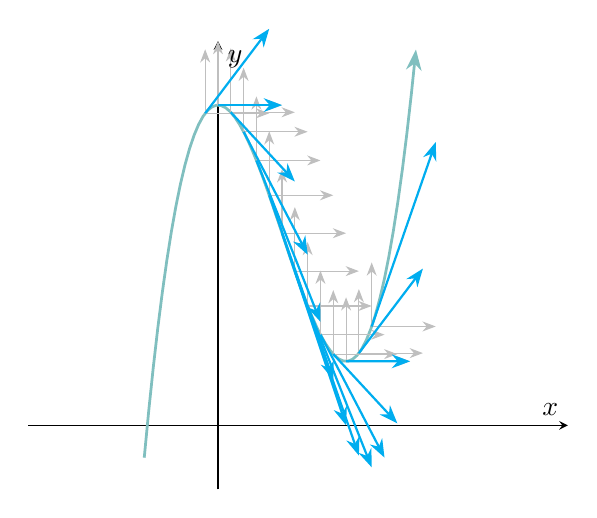
\begin{tikzpicture}
\begin{axis}[
axis lines=center,
xlabel={$x$}, ylabel={$y$},
xtick=\empty, ytick=\empty,
xmin=-2.5, xmax=5,   % Adjusted axis limits
ymin=-1, ymax=6,    % Adjusted axis limits
restrict y to domain=-1:6,
axis equal, % Ensures slopes are visually correct
clip=false
]
\addplot[-{Stealth}, domain=-2:5, samples=100, line width=.35mm, teal!50] {((x+1)*(x-2)*(x-2) + 1} node[right] {};
\pgfplotsextra{
	\foreach \a in {-.2, 0, ..., 2.4} {
		\pgfmathsetmacro{\dx}{1}
		
		% Compute f(a) = a^3 - 3a^2 + 5
		\pgfmathparse{\a*\a*\a - 3*\a*\a + 5}
		\edef\ay{\pgfmathresult}
		% Coordinates
		\edef\coordx{
			\noexpand\draw[-Stealth, gray!50]
			(axis cs:\a,\ay) -- (axis cs:\a+1,\ay); 
			%			node[right] {$\langle 1, f'(\a)\rangle$};
		}
		\coordx
		\edef\coordy{
			\noexpand\draw[-Stealth, gray!50]
			(axis cs:\a,\ay) -- (axis cs:\a,\ay+1); 
			%			node[right] {$\langle 1, f'(\a)\rangle$};
		}
		\coordy
	}
}
% Tangent vectors from point a
\pgfplotsextra{
	\foreach \a in {-.2, 0, ..., 2.4} {
		\pgfmathsetmacro{\dx}{1}
		
		% Compute f(a) = a^3 - 3a^2 + 5
		\pgfmathparse{\a*\a*\a - 3*\a*\a + 5}
		\edef\ay{\pgfmathresult}
		
		% Compute f'(a) = 3a^2 - 6a
		\pgfmathparse{3*\a*\a - 6*\a}
		\edef\slope{\pgfmathresult}
		
		% Compute vector end point (a+dx, f(a)+slope*dx)
		\pgfmathparse{\a + \dx} \edef\endx{\pgfmathresult}
		\pgfmathparse{\ay + \slope*\dx} \edef\endy{\pgfmathresult}
		
		% Draw arrow
		\edef\cmd{
			\noexpand\draw[-{Stealth}, thick, cyan]
			(axis cs:\a,\ay) -- (axis cs:\endx,\endy); 
%			node[right] {$\langle 1, f'(\a)\rangle$};
		}
		\cmd
		
		% Coordinates
%		\edef\coordx{
%			\noexpand\draw[-Stealth, gray]
%			(axis cs:\a,\ay) -- (axis cs:{\a},0); 
%			%			node[right] {$\langle 1, f'(\a)\rangle$};
%		}
%		\coordx
%		\edef\coordy{
%			\noexpand\draw[-Stealth, gray]
%			(axis cs:\a,\ay) -- (axis cs:0,\ay); 
%			%			node[right] {$\langle 1, f'(\a)\rangle$};
%		}
%		\coordy
	}
}
\end{axis}
\end{tikzpicture}
\end{document}
